\section{Database and selection of test subjects}
As test sample a data set of XXX\todo{how many?} ICAO compliant pictures were given. In order to get promising morph results, a subset of XX \todo{number} pairs of photos were selected for manual morphing \ref{manual_morph} where as the automatic morphing algorithm \ref{automatic_morph} was applied on all data sets. For manual  morphing only pairs with a visually high coincidence are considered because the aceptance rate of the comparison algorithem is expected to be higher. 
In summation XX manual and XXX automatic morphs are issued in this paper. 

\todo[inline]{ICAO conformance beschrieben}
\todo[inline]{FaceDB}

\section{Morphing of Faces}
The main task during the morphing of two pictures is to detect characteristics and place landmarks as an advince for the algorithm. This can be done completely automatic or with support of an user. In this paper both way are discussed.  
\subsection{Basic idea}
\label{percentageMorph}
For every morph there were 15 images created from 0\% of Subject 1 to 100\%, respectively the remaining \% of Person 2. So the are images combined of:
\begin{itemize}
	\item 1. Picture: Person 1 100\% - Person 2 0\%
	\item 2. Picture: Person 1 92,86\% - Person 2 7,14\%
	\item 3. Picture: Person 1 85,71\% - Person 2 14,29\%
	\item 4. Picture: Person 1 78,57\% - Person 2 21,43\%
	\item 5. Picture: Person 1 71,43\% - Person 2 28,57\%
	\item 6. Picture: Person 1 64,29\% - Person 2 35,71\%
	\item 7. Picture: Person 1 57,14\% - Person 2 42,86\%
	\item 8. Picture: Person 1 50,00\% - Person 2 50,00\%
	\item 9. Picture: Person 1 42,86\% - Person 2 57,14\%
	\item 10. Picture: Person 1 35,71\% - Person 2 64,29\%
	\item 11. Picture: Person 1 28,57\% - Person 2 71,43\%
	\item 12. Picture: Person 1 21,43\% - Person 2 78,57\%
	\item 13. Picture: Person 1 14,29\% - Person 2 85,71\%
	\item 14. Picture: Person 1 7,14\% - Person 2 92,86\%
	\item 15. Picture: Person 1 0\% - Person 2 100\%
	\end{itemize}

\todo[inline]{say something on this + make tabular}
\subsection{Automatic morphing}
\label{automatic_morph}


\subsection{Manual morphing}
\label{manual_morph}
\begin{figure}[h]
	\centering
	\subfloat[Subject 1]{%
		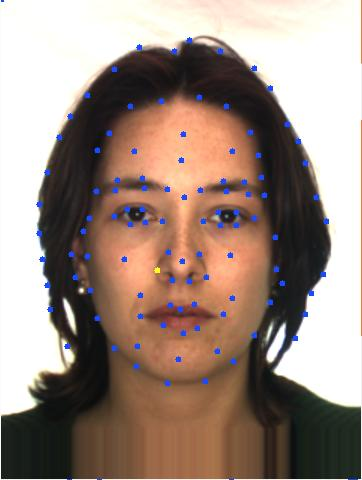
\includegraphics[width=0.25\linewidth]{Resources/manualmorph01.jpg}}
	\label{subfig:manualmorph01}\hfill
	\subfloat[Morph no. 5]{%
		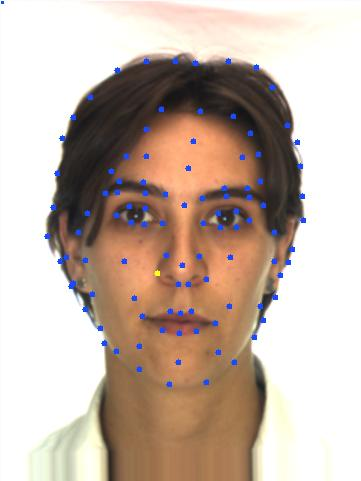
\includegraphics[width=0.25\linewidth]{Resources/manualmorph02.jpg}}
	\label{subfig:manualmorph02}\\
	\caption{Example of two ICAO compliant photos (1a and 1e) and morphs at stage 5 (1b), 15 (1c) and 25 (1d)}
	\label{fig:manual_morph} 
\end{figure}
In contrast to the automatic face morphing approach, manual morphing is discussed in this section. 

To achieve morphes, the open source software GNU Image Manipulation Software (GIMP) (Version 2.8.16) with the GIMP Animation Package (GAP) (Version 2.6) was selected for this process. Morphing with GAP follows the simple approach of manually placing connected landmarks at characterizing points in both faces. In \ref{fig:manual_morph} two pictures with a setup of landmarks are shown. It can be observed, that the landmarks are placed at characterizing points in both faces, e.g. at the eye browns, lips and nose. The general shape of the face as well as the shape of the head including the hair is also respected. In the example the facial landmarks are close to each other whereas the landmarks describing the shape of the hair are farer apart. 

The selection of characterizing points \todo{regions?}is based on *erkenntnissen* from earlier works on the topic of automatic face recognition, to achieve an optimal morphing result compared with own estimasation based on the individual appeance of the subjects. \todo{cite handbook of bio p.60} \todo{cite these fancy mp4 thingy}. 

\cite{vukadinovic2005fully}



The algorithm shifts the landmarks from face one to face two. In addition to this the color of the skin is transmitted. 

%\subsubsection*{Morphing setup}
For the test samples 100 - 125 landmarks were placed, depending on the face characteristics. The output contains a sequence of 30 photos which show different stages of the morphing procedure. \ref{1e}


\subsubsection*{Results}
\todo{compare to automatic results when there.}
\begin{figure}[h]
	\centering
	\subfloat[Subject 1]{%
		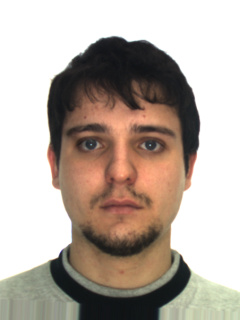
\includegraphics[width=0.30\linewidth]{Resources/p1.jpg}
	\label{1a}}\hfill
	\subfloat[Morph no. 5]{%
		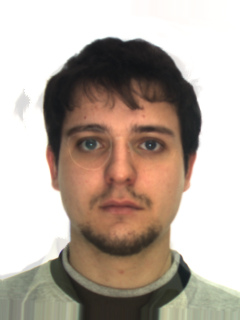
\includegraphics[width=0.30\linewidth]{Resources/m1.jpg}
	\label{foo}}\\
	\subfloat[Morph no. 15]{%
		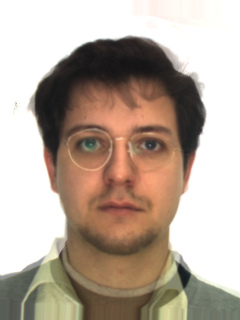
\includegraphics[width=0.30\linewidth]{Resources/m2.jpg}
	\label{1c}} \hfill
	\subfloat[Morph no. 25]{%
		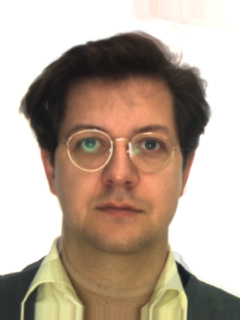
\includegraphics[width=0.30\linewidth]{Resources/m3.jpg}
	\label{1d}}\hfill
	\subfloat[Subject 2]{%
		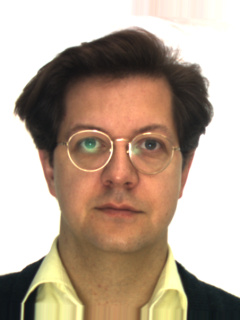
\includegraphics[width=0.30\linewidth]{Resources/p2.jpg}
	\label{1e} }
	\caption{Example of two ICAO compliant photos (1a and 1e) and morphs at stage 5 (1b), 15 (1c) and 25 (1d)}
	\label{fig1} 
\end{figure}

In figure \ref{fig1} a two subjects and three morphing stages (5, 15 and 25) are shown. The visual inspection of \ref{1a} shows biometric features of both subjects whereas \subref{1e} and \ref{1d} has more similarity to the closer subject but also covers features of the other subject.
A manual post production of the morphs is not necessary because potential revealing details, like the interference \todo{?} of the clothes, glasses or hair is not considered by the algorithm.

\todo[inline]{Detailed description of the morphs}